\section{Introduction}
High software quality is one of the most important goal of software development. Software testing serves as the most widely used approach to ensure the quality of softwares meet expectation.
%Software testing is one of the most important processes in HPC software development. 
A good way to test software is to include automated tests in the build process.  With the rise of Extreme Programming (XP) and Test Driven Development (TDD), self-testing processes for code development have become popular and are widely adopted by many software development projects. 
As softwares become increasingly structurally complicated, the number of developers involved in the development process increases. As each developer makes progress, they commit their work periodically (every several hours or days) to the central code repository (e.g., git, SVN). Not only does each developer's work require testing, the integration of work between developers also requires testing. So, Continuous Integration (CI) \cite{fowler2006continuous} is widely adopted in many software development projects. A CI server is used dedicatedly for testing. Each time a developer makes a commit of her work to the central code repository, the CI server automatically make a clone of the project and conduct pre-designed tests, so that it can constantly monitor the quality of the software in terms of correctness and report potential problems in a timely fashion, helping developers make bug fixes more efficiently.  %\pat{I wouldn't say the servers mimic the production env.}
%\pat{what is this a hanging here for}

\begin{figure*}[h]
    \centering
    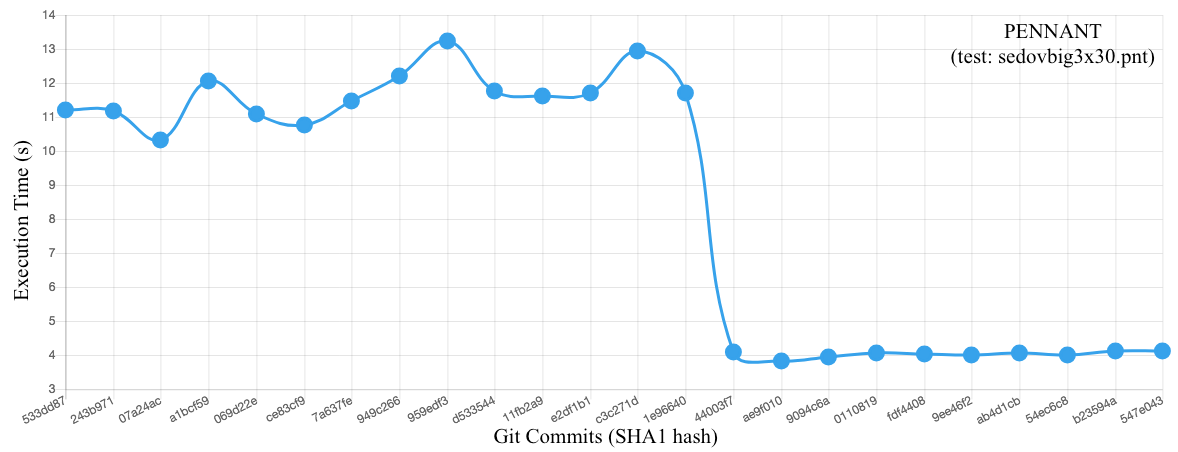
\includegraphics[width=1\textwidth]{figures/CI-motivation-2.png}
    \caption{Example: the performance of Legion \cite{bauer2012legion} changes as developers make progress. The performance is obtained by running a benchmark PENNANT\cite{ferenbaugh2015pennant} on the Legion system. The test suit sedovbig3x30 running on 10 processes (CPU cores) is used. 
%\textcolor{red}{Caption should be changed because this perforamnce is about Legion not PENNANT.}
}
    \label{exp}
\end{figure*}


When it comes to HPC applications, \textit{performance} and \textit{scalability} %large-scale
%\trandles{Remove 'large-scale' here because you have it at the end of the sentence} 
are the other two important factors of software quality besides correctness, since the application are usually designed to deliver high performance on given platforms. Also applications that aim to solve complex time-consuming problems are expected to obtain good speedup when deployed on multi-node clusters, many-core architectures, or large-scale supercomputers. The scalability of HPC application is usually interpreted as how much speed up can be obtained given more computing resources. Better scalability means that the HPC application can use the underlying computing resources more efficiency and constantly deliver good performance on a various amount of computing resources.

During the HPC application development, as developers make progress,
%\pat{not sure if I changed your meaning here}
and they commit their work to the central code repository, the scalability of the application can change. For instance, it can be caused by changes in algorithm design, tunable parameters, and different hardware architectures of target production systems. For example, \textbf{Fig. \ref{exp}} shows the  performance of Legion \cite{bauer2012legion}, a data-centric parallel programming system, changes %\pat{shouldn't you explain what Circuit is I assume it's some sort of simulation, is it really an HPC code or just a benchmark code? Also, the axes of figure need to be labels I have no idea what they are}
%\trandles{Change the data point styles on the graph and refer to them by the symbols instead of colors.  Color-blind readers won't be able to easily distinguish between the two data series as presented.}
with different source code commits. The performance is obtained by running a benchmark software, PENNANT\cite{ferenbaugh2015pennant}, on the Legion system. As we can see the execution time can significantly change as developers make progresses. Receiving performance or scalability results like this in a timely manner can greatly help developers make better decisions about their code design and deliver HPC software with expected quality. However, current designs of CI services are commonly focused on monitoring the software quality in terms of correctness (e.g., detecting software bugs). To the best of our knowledge, none of the current works can easily enable automatic performance or scalability tests in CI since the test environment of CI is usually deployed on a single machine incapable of conducting large-scale scalability test.

\begin{figure}[h]
    \centering
    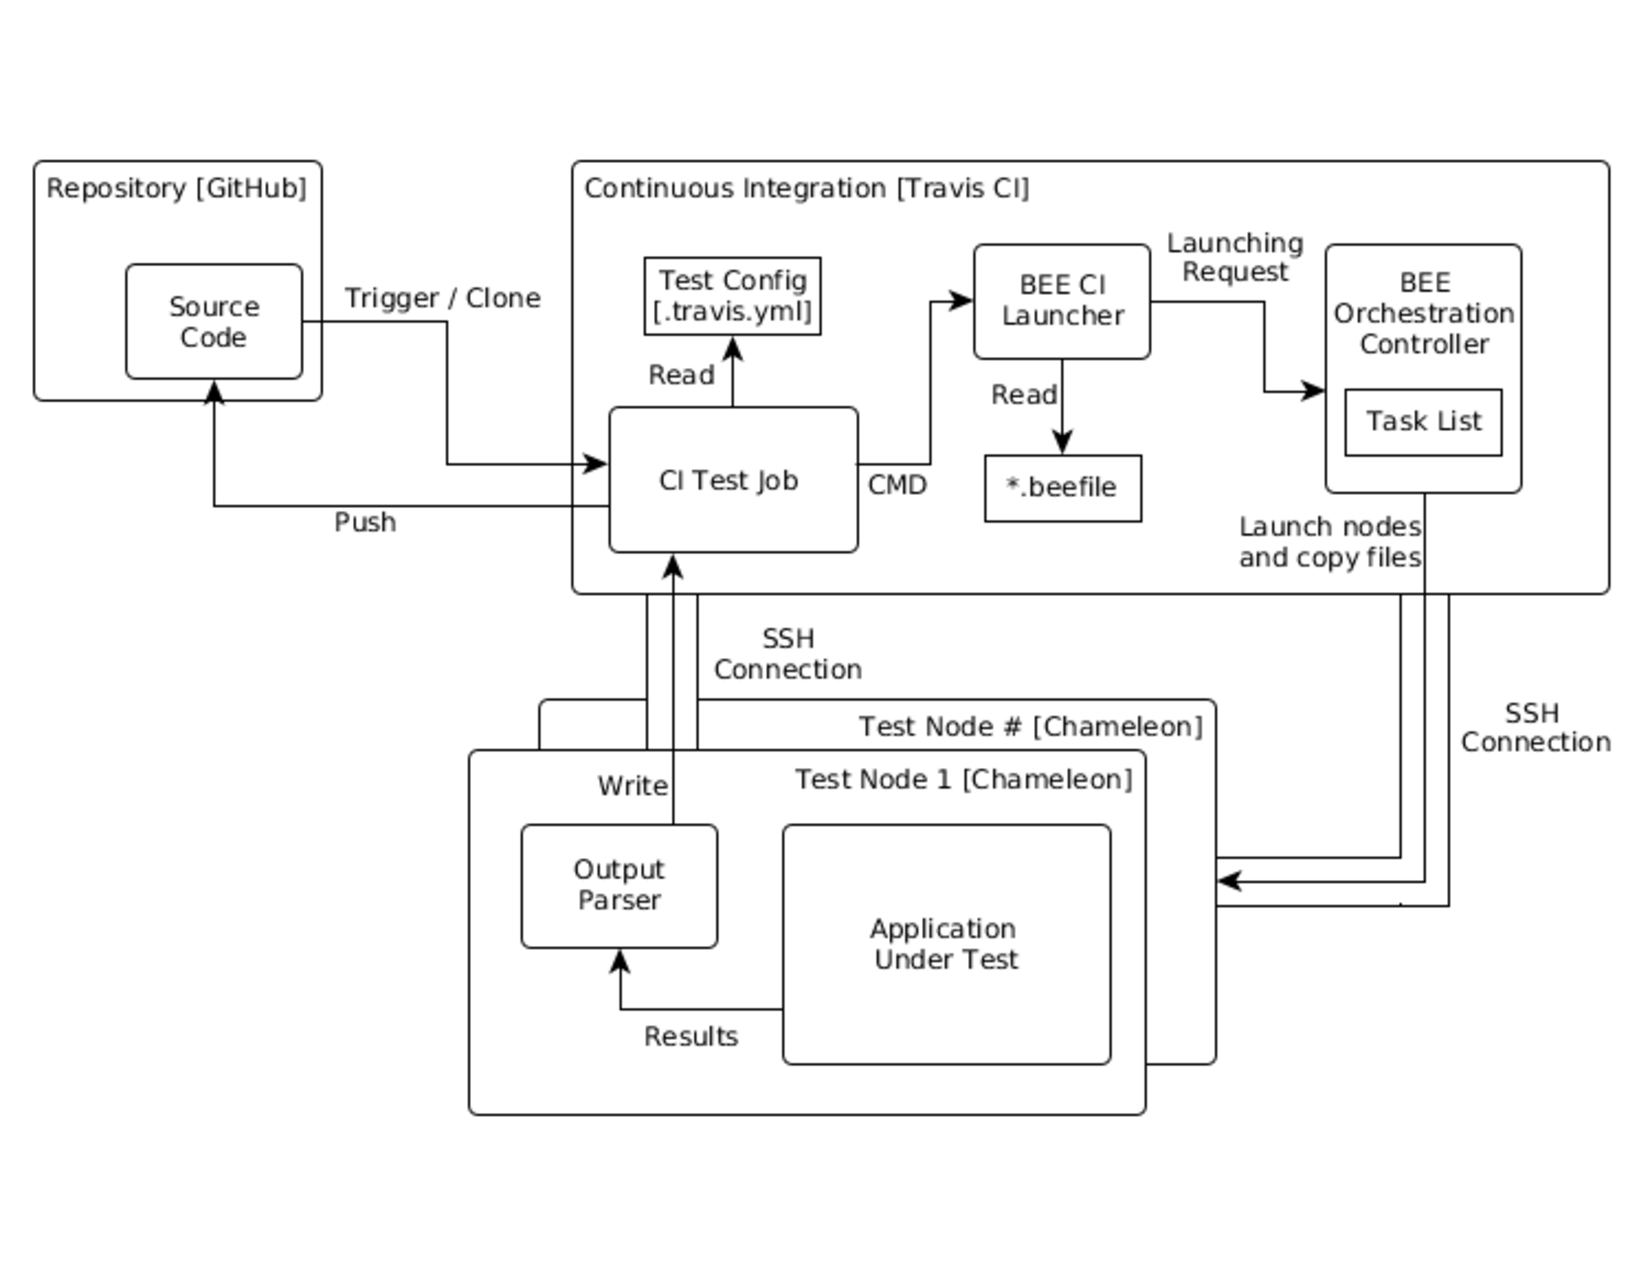
\includegraphics[width=0.5\textwidth]{figures/beeSwarm_Arch_ver02.pdf}
    \caption{Architecture of \texttt{BeeSwarm}. %\textcolor{red}{****Figure is not readable}
    }
    \label{arch}
\end{figure}


In this work, we propose a performance and scalability test system for CI -- \texttt{BeeSwarm}. \texttt{BeeSwarm} can be used as a plug-in for any current CI service. It takes the widely used Docker container as input, and the performance and scalability test can run on both HPC cluster environments and cloud computing environments. Just like the original correctness test in CI, the performance and scalability test are also autonomic. It only requires users to make simple specifications about the test environment they want to use and the test specification they need. Every time developers commit a change to the central code repository, they can choose to schedule a scalability test after the success of original correctness test. The performance and scalability test results will be automatically pushed back to the central code repository. %\pat{can this be controlled, maybe they don't want every change to spawn a scalability test}
Although we deploy \texttt{BeeSwarm} on Travis CI in this work, it can also be deployed on any other CI test environment. To deploy on another CI platform, only minimum modifications to the \texttt{BeeSwarm} configuration scripts are necessary, which makes \texttt{BeeSwarm} highly portable across CI platforms. In addition, although we only show the use of Chameleon cloud, the scalability test can also be executed on any other BEE-supported platform (HPC clusters, AWS, OpenStack, etc). This gives developers the flexibility to choose the platform they want their applications to run on.

The rest of this paper is organized as follows. We motivate our work in section \ref{motivation}. In section \ref{background}, we give necessary background that can help readers understand this work. We provide design details of \texttt{BeeSwarm} in section \ref{design} followed by experimental evaluation in section \ref{experiments}. Section \ref{related_work} discuss recent works that related to ours. Finally, section \ref{conclusion} concludes our work. %\textcolor{red}{Please change this accordingly after adding the motivation session}

\begin{figure*}[h]
    \centering
    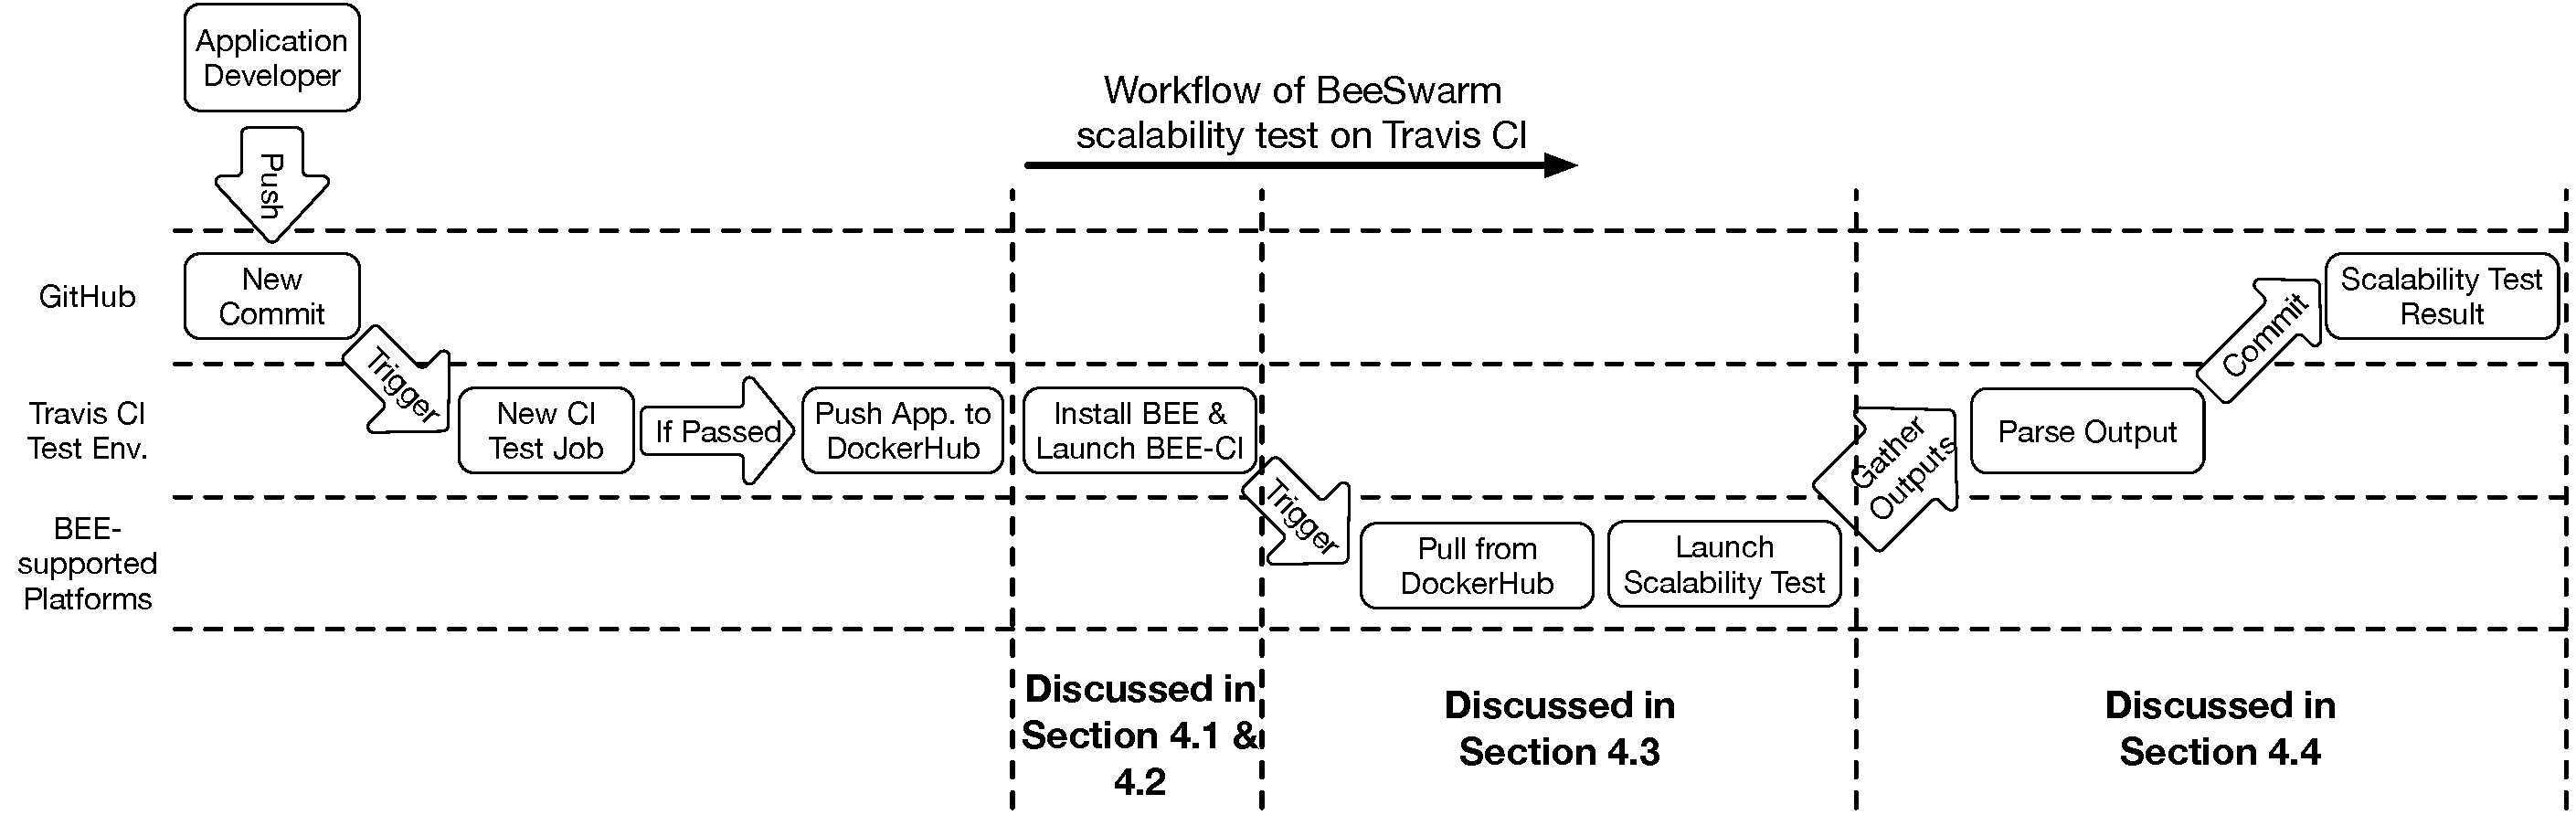
\includegraphics[width=1\textwidth]{figures/CI-workflow.pdf}
    \caption{Overall Workflow of BeeSwarm CI Scalability Test. 
    %\textcolor{red}{Can we add some horizontal lines to partition the steps of workflow to make them mapping 4.1-4.4? And move this graph to page 3, on top of it.}
    }
    \label{overall}
\end{figure*}